%%%%%%%%%%%%%%%%%%%%%%%%%%%%%%%%%%%%%%%%%
% Jacobs Portrait Poster
% LaTeX Template
% Version 1.0 (31/08/2015)
% (Based on Version 1.0 (29/03/13) of the landscape template
%
% Created by:
% Computational Physics and Biophysics Group, Jacobs University
% https://teamwork.jacobs-university.de:8443/confluence/display/CoPandBiG/LaTeX+Poster
% 
% Further modified by:
% Nathaniel Johnston (nathaniel@njohnston.ca)
%
% Portrait version by:
% John Hammersley
%
% The landscape version of this template was downloaded from:
% http://www.LaTeXTemplates.com
%
% License:
% CC BY-NC-SA 3.0 (http://creativecommons.org/licenses/by-nc-sa/3.0/)
%
%%%%%%%%%%%%%%%%%%%%%%%%%%%%%%%%%%%%%%%%%

%----------------------------------------------------------------------------------------
%	PACKAGES AND OTHER DOCUMENT CONFIGURATIONS
%----------------------------------------------------------------------------------------

\documentclass[final]{beamer}

\usepackage[scale=1.24]{beamerposter} % Use the beamerposter package for laying out the poster
\usepackage{siunitx}

\usetheme{confposter} % Use the confposter theme supplied with this template

\setbeamercolor{block title}{fg=Cerulean,bg=white} % Colors of the block titles
\setbeamercolor{block body}{fg=black,bg=white} % Colors of the body of blocks
\setbeamercolor{block alerted title}{fg=white,bg=Cerulean!60} % Colors of the highlighted block titles
\setbeamercolor{block alerted body}{fg=black,bg=Cerulean!10} % Colors of the body of highlighted blocks
% Many more colors are available for use in beamerthemeconfposter.sty

%-----------------------------------------------------------
% Define the column widths and overall poster size
% To set effective sepwid, onecolwid and twocolwid values, first choose how many columns you want and how much separation you want between columns
% In this template, the separation width chosen is 0.024 of the paper width and a 4-column layout
% onecolwid should therefore be (1-(# of columns+1)*sepwid)/# of columns e.g. (1-(4+1)*0.024)/4 = 0.22
% Set twocolwid to be (2*onecolwid)+sepwid = 0.464
% Set threecolwid to be (3*onecolwid)+2*sepwid = 0.708

\newlength{\sepwid}
\newlength{\onecolwid}
\newlength{\twocolwid}
\newlength{\threecolwid}
\setlength{\paperwidth}{36in} % A0 width: 46.8in
\setlength{\paperheight}{48in} % A0 height: 33.1in
% \setlength{\sepwid}{0.024\paperwidth} % Separation width (white space) between columns
% \setlength{\onecolwid}{0.22\paperwidth} % Width of one column
% \setlength{\twocolwid}{0.464\paperwidth} % Width of two columns
% \setlength{\threecolwid}{0.708\paperwidth} % Width of three columns
\setlength{\sepwid}{0.022\paperwidth} % Separation width (white space) between columns
\setlength{\onecolwid}{0.304\paperwidth} % Width of one column
\setlength{\twocolwid}{0.63\paperwidth} % Width of two columns
\setlength{\threecolwid}{0.956\paperwidth} % Width of three columns
\setlength{\topmargin}{-1in} % Reduce the top margin size
%-----------------------------------------------------------

\usepackage{graphicx}  % Required for including images

\usepackage{booktabs} % Top and bottom rules for tables

%----------------------------------------------------------------------------------------
%	TITLE SECTION 
%----------------------------------------------------------------------------------------

\title{A Portable Real-Time Polarimeter by the \\ Use of the Spinning Waveplate Method} % Poster title

\author{Julian Nicolai, Wilfrid-Shaun Nortey-Noye, \\  Brendan Ford, and Adam Thomson} % Author(s)

\institute{Department of Electronics, Carleton University} % Institution(s)

%----------------------------------------------------------------------------------------

\begin{document}

\addtobeamertemplate{block end}{}{\vspace*{2ex}} % White space under blocks
\addtobeamertemplate{block alerted end}{}{\vspace*{2ex}} % White space under highlighted (alert) blocks

\setlength{\belowcaptionskip}{2ex} % White space under figures
\setlength\belowdisplayshortskip{2ex} % White space under equations

\begin{frame}[t] % The whole poster is enclosed in one beamer frame

\begin{columns}[t] % The whole poster consists of three major columns, the second of which is split into two columns twice - the [t] option aligns each column's content to the top

% \begin{tikzpicture}[remember picture, overlay]
%     \node [shift={(5in, -1.9in)}] at (current page.north west)
%         { 
\includegraphics[width=8in]{Images/misc/intempco_logo.png} };
% \end{tikzpicture}

% \begin{tikzpicture}[remember picture, overlay]
%     \node [shift={(5in, -4.4in)}] at (current page.north west)
%         { \includegraphics[width=8in]{Images/misc/nrc_logo.png} };
% \end{tikzpicture}

\begin{tikzpicture}[remember picture, overlay]
    \node [shift={(-5in, -5.1in)}] at (current page.north east)
        { 
\includegraphics[width=8in]{Images/misc/carleton_logo.png} };
\end{tikzpicture}

% \begin{tikzpicture}[remember picture, overlay]
%     \node [shift={(5in, -5.1in)}] at (current page.north west)
%         { \includegraphics[width=8in]{Images/misc/carleton_logo_v2.jpg} };
% \end{tikzpicture}

% \begin{tikzpicture}[remember picture, overlay]
%     \node [shift={(-4in, -5.1in)}] at (current page.north east)
%         { 
\includegraphics[width=6in]{Images/misc/doe_logo.jpg} };
% \end{tikzpicture}

\begin{tikzpicture}[remember picture, overlay]
    \node [shift={(4in, -5.1in)}] at (current page.north west)
        { 
\includegraphics[width=6in]{Images/misc/doe_logo.jpg} };
\end{tikzpicture}

\begin{column}{\sepwid}\end{column} % Empty spacer column

\begin{column}{\onecolwid} % The first column

%----------------------------------------------------------------------------------------
% COLUMN 1
%----------------------------------------------------------------------------------------

% ======= Introduction ==================================================================

\begin{block}{Introduction}

Lorem ipsum dolor sit amet, consectetur adipiscing elit. Sed turpis leo, egestas a mi et, pharetra fringilla risus. Sed lacinia felis ut feugiat laoreet. Interdum et malesuada fames ac ante ipsum primis in faucibus. Cras leo.

\end{block}
\vspace{-0.3in}

% ======= Tilted FBG's ==================================================================

\begin{block}{Section 1}

Lorem ipsum dolor sit amet, consectetur adipiscing elit. Cras a ex commodo, venenatis est ullamcorper, accumsan sapien. Sed diam turpis, tempus a congue at, finibus et arcu. Phasellus iaculis, massa sed feugiat euismod, quam sem eleifend ligula, ut tincidunt mi elit vitae nibh. Mauris erat nibh, gravida eget dui in, vestibulum laoreet enim. Vestibulum aliquet commodo nulla, non faucibus nunc semper ut.

\end{block}

\begin{figure}
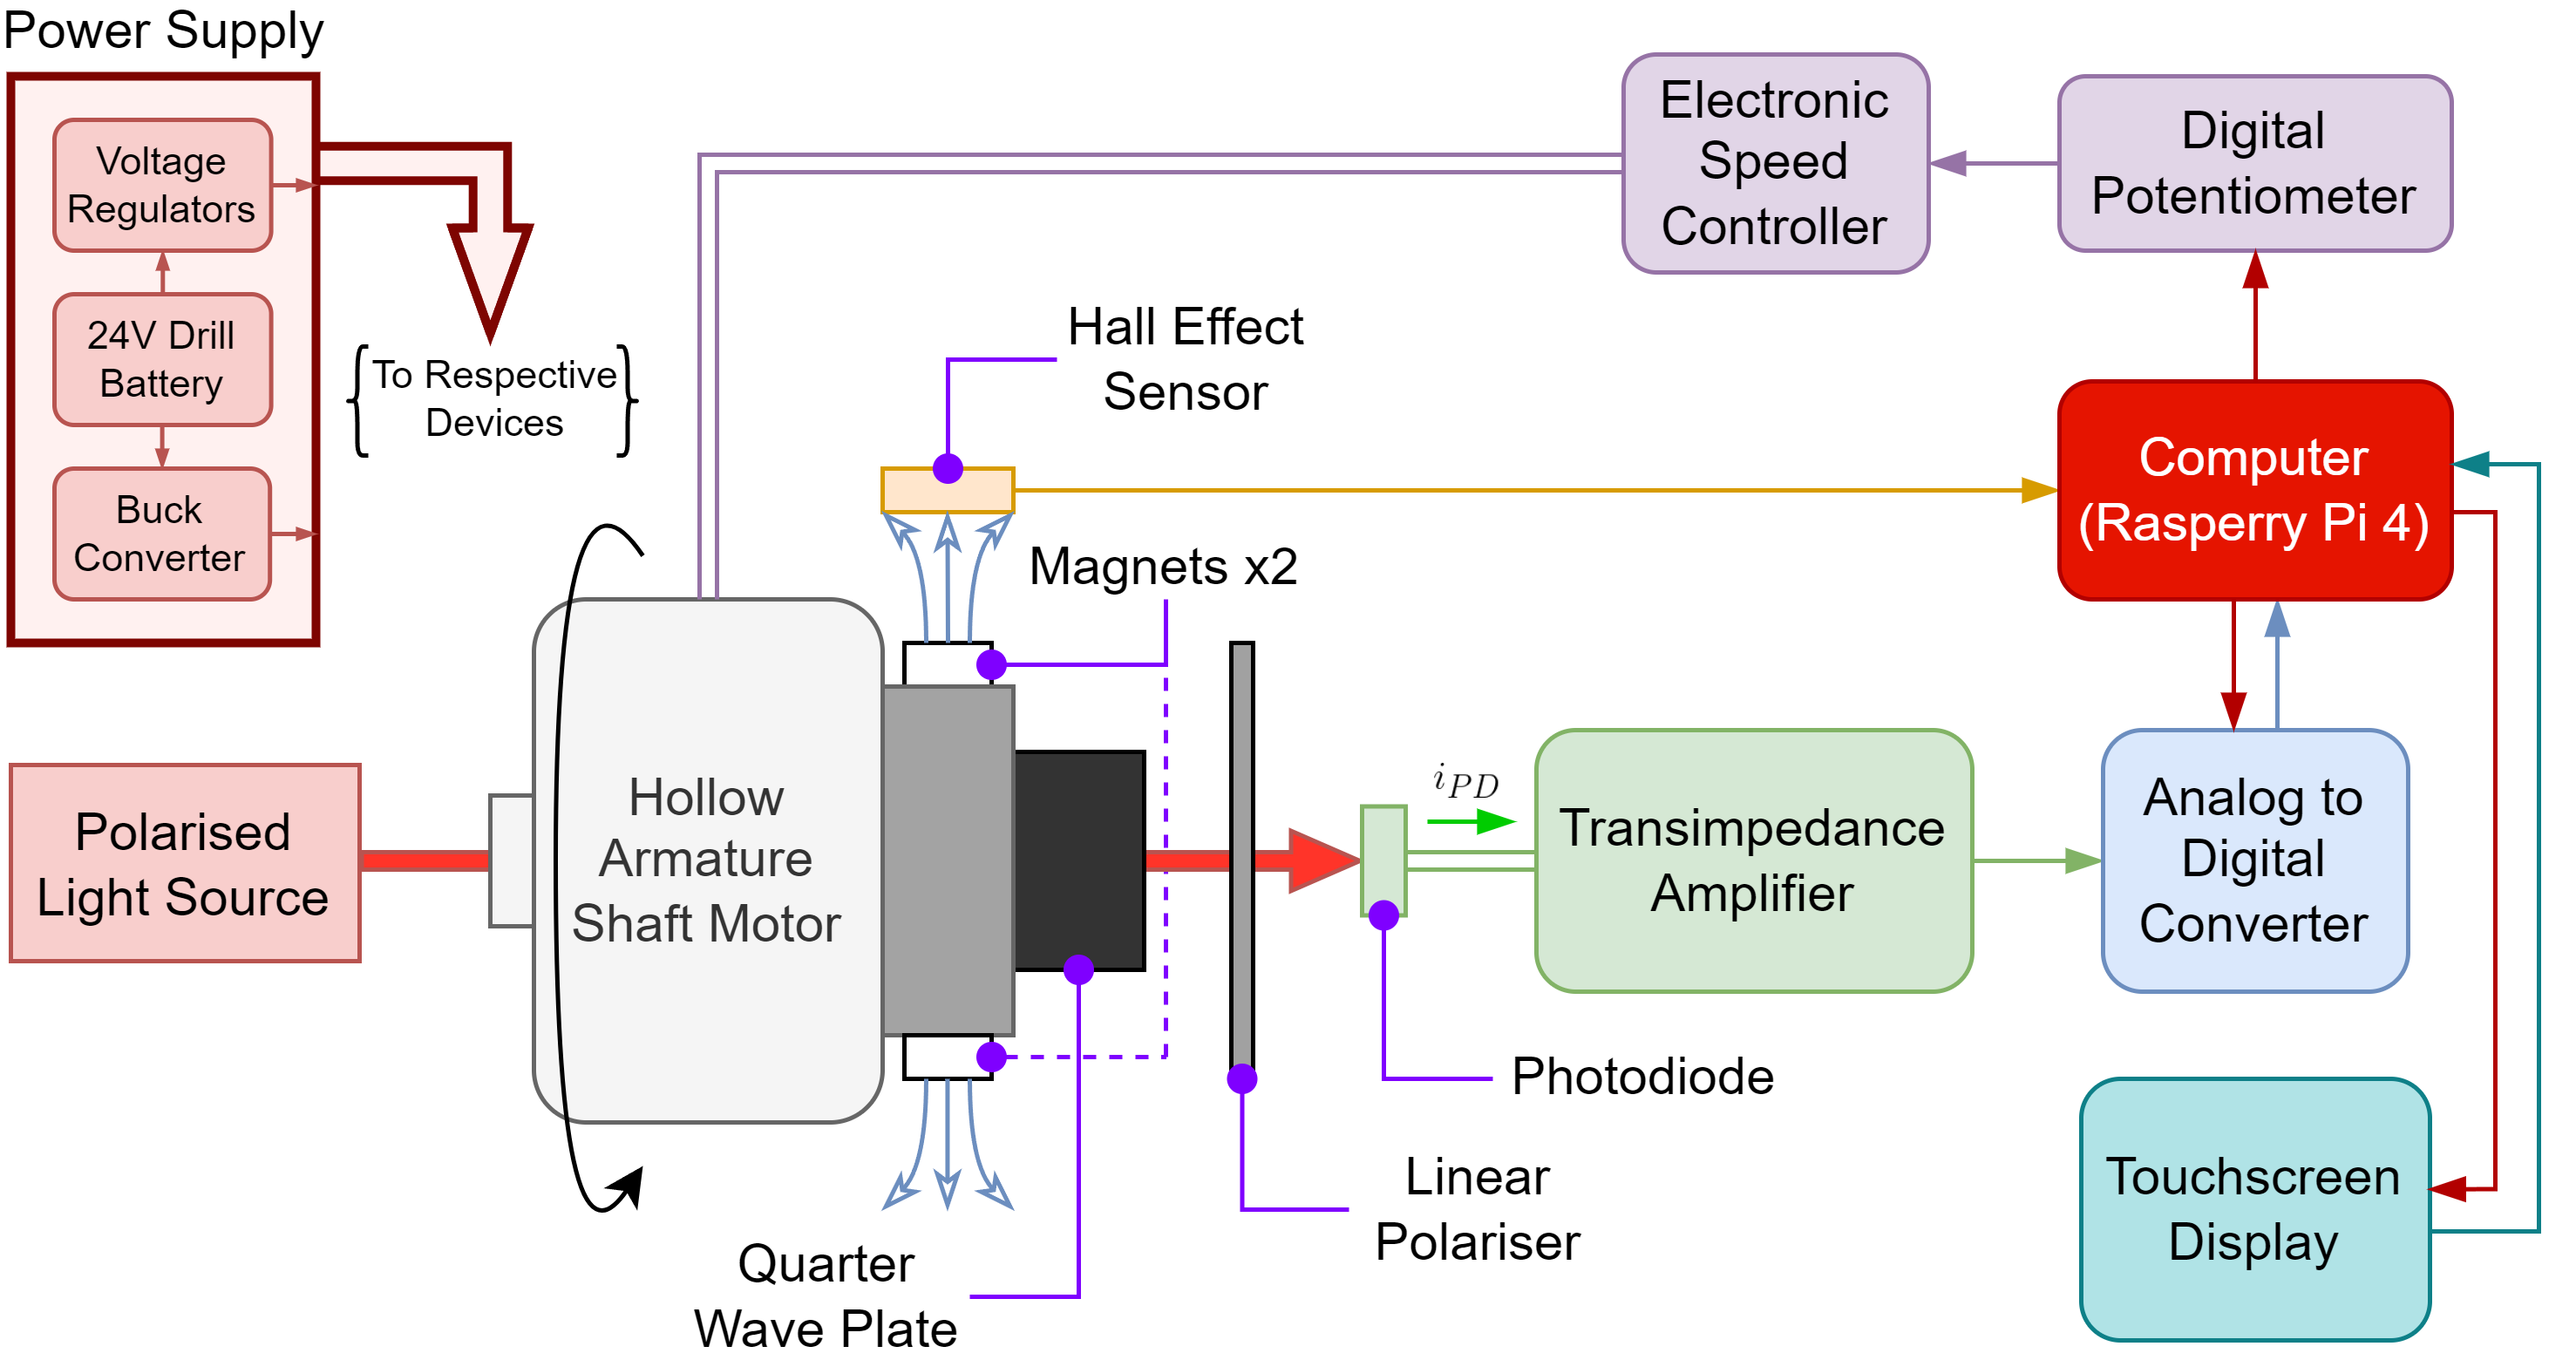
\includegraphics[width=1\linewidth]{Images/FunctionalDiagram.png}
\caption{Labelled tilted FBG diagram; operating principles and dimensions.}
\end{figure}

%  ======= Contour Length Analysis ========================================================

\begin{alertblock}{Highlight Section}

Lorem ipsum dolor sit amet, consectetur adipiscing elit. Fusce in nisi orci. Proin maximus varius fermentum. Nunc eu lacinia elit. In hac sed \cite{Wawrzyk_2022}. 

\begin{equation}
    L = \Sigma_{i=0}^{N-1} |P_{i+1} - P_{i}|
    \label{equ:contlen}
\end{equation}

\begin{figure}
    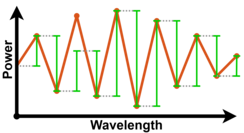
\includegraphics[width=0.75\linewidth]{Images/calc_contour_length_v2_LQ.png}
    \caption{The sum of the green lines is the contour length.}
\end{figure}

Lorem ipsum dolor sit amet, consectetur adipiscing elit. Morbi sed ipsum nec massa interdum malesuada non ac nulla. In vitae urna in ante sollicitudin tempor in eu eros. Sed condimentum, magna quis efficitur vestibulum, purus erat accumsan sem, eu interdum est sapien elementum dui. Suspendisse viverra.

\end{alertblock}

\vspace*{0.4in}

\setbeamercolor{block alerted title}{fg=black,bg=FuckingShinoBro} % Change the alert block title colors
\setbeamercolor{block alerted body}{fg=black,bg=FuckingShinoBro!10} % Change the alert block body colors

\begin{alertblock}{Alert Section}

Lorem ipsum dolor sit amet, consectetur adipiscing elit. Fusce in nisi orci. Proin maximus varius fermentum. Nunc eu lacinia elit. In hac sed.

% \vspace*{0.2in}
% \begin{center}
% \begin{tabular}{ccc}
% 
\includegraphics[height=1.7in]{Images/misc/nserc_logo.png} & \hspace*{0.5in} & 
\includegraphics[height=1.7in]{Images/misc/intempco_logo.png}
% \end{tabular}
% \end{center}

\end{alertblock}

\setbeamercolor{block alerted title}{fg=white,bg=Cerulean}
\setbeamercolor{block alerted body}{fg=black,bg=Cerulean}

%----------------------------------------------------------------------------------------

\end{column} % End of the first column

\begin{column}{\sepwid}\end{column} % Empty spacer column

\begin{column}{\onecolwid} % Begin a column which is two columns wide (column 2)

%----------------------------------------------------------------------------------------
% COLUMN 2
%----------------------------------------------------------------------------------------

%  ======= Bend Sensing =================================================================

\begin{block}{Section 2}

Lorem ipsum dolor sit amet, consectetur adipiscing elit. Sed blandit massa id maximus tristique. Curabitur eget viverra sem. Quisque sit amet rhoncus elit. Nunc accumsan eros dui, nec tincidunt tortor interdum condimentum. Fusce tincidunt eget turpis eu eleifend. Nullam aliquam quam amet.

\end{block}
\vspace{-0.3in}

\begin{figure}
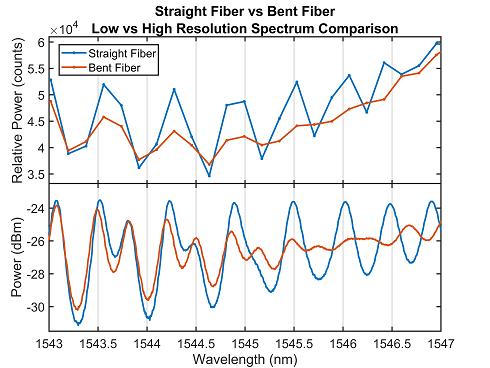
\includegraphics[width=1\linewidth]{Images/bending_spectrum_v4_HD_v2_LQ.png}
\caption{When bending is introduced to a \SI{3}{\milli\metre}, $4^{\circ}$ TFBG the peak prominence decreases. This phenomena can still be observed using low-resolution equipment.}
\end{figure}
\vspace{-0.3in}

\begin{figure}
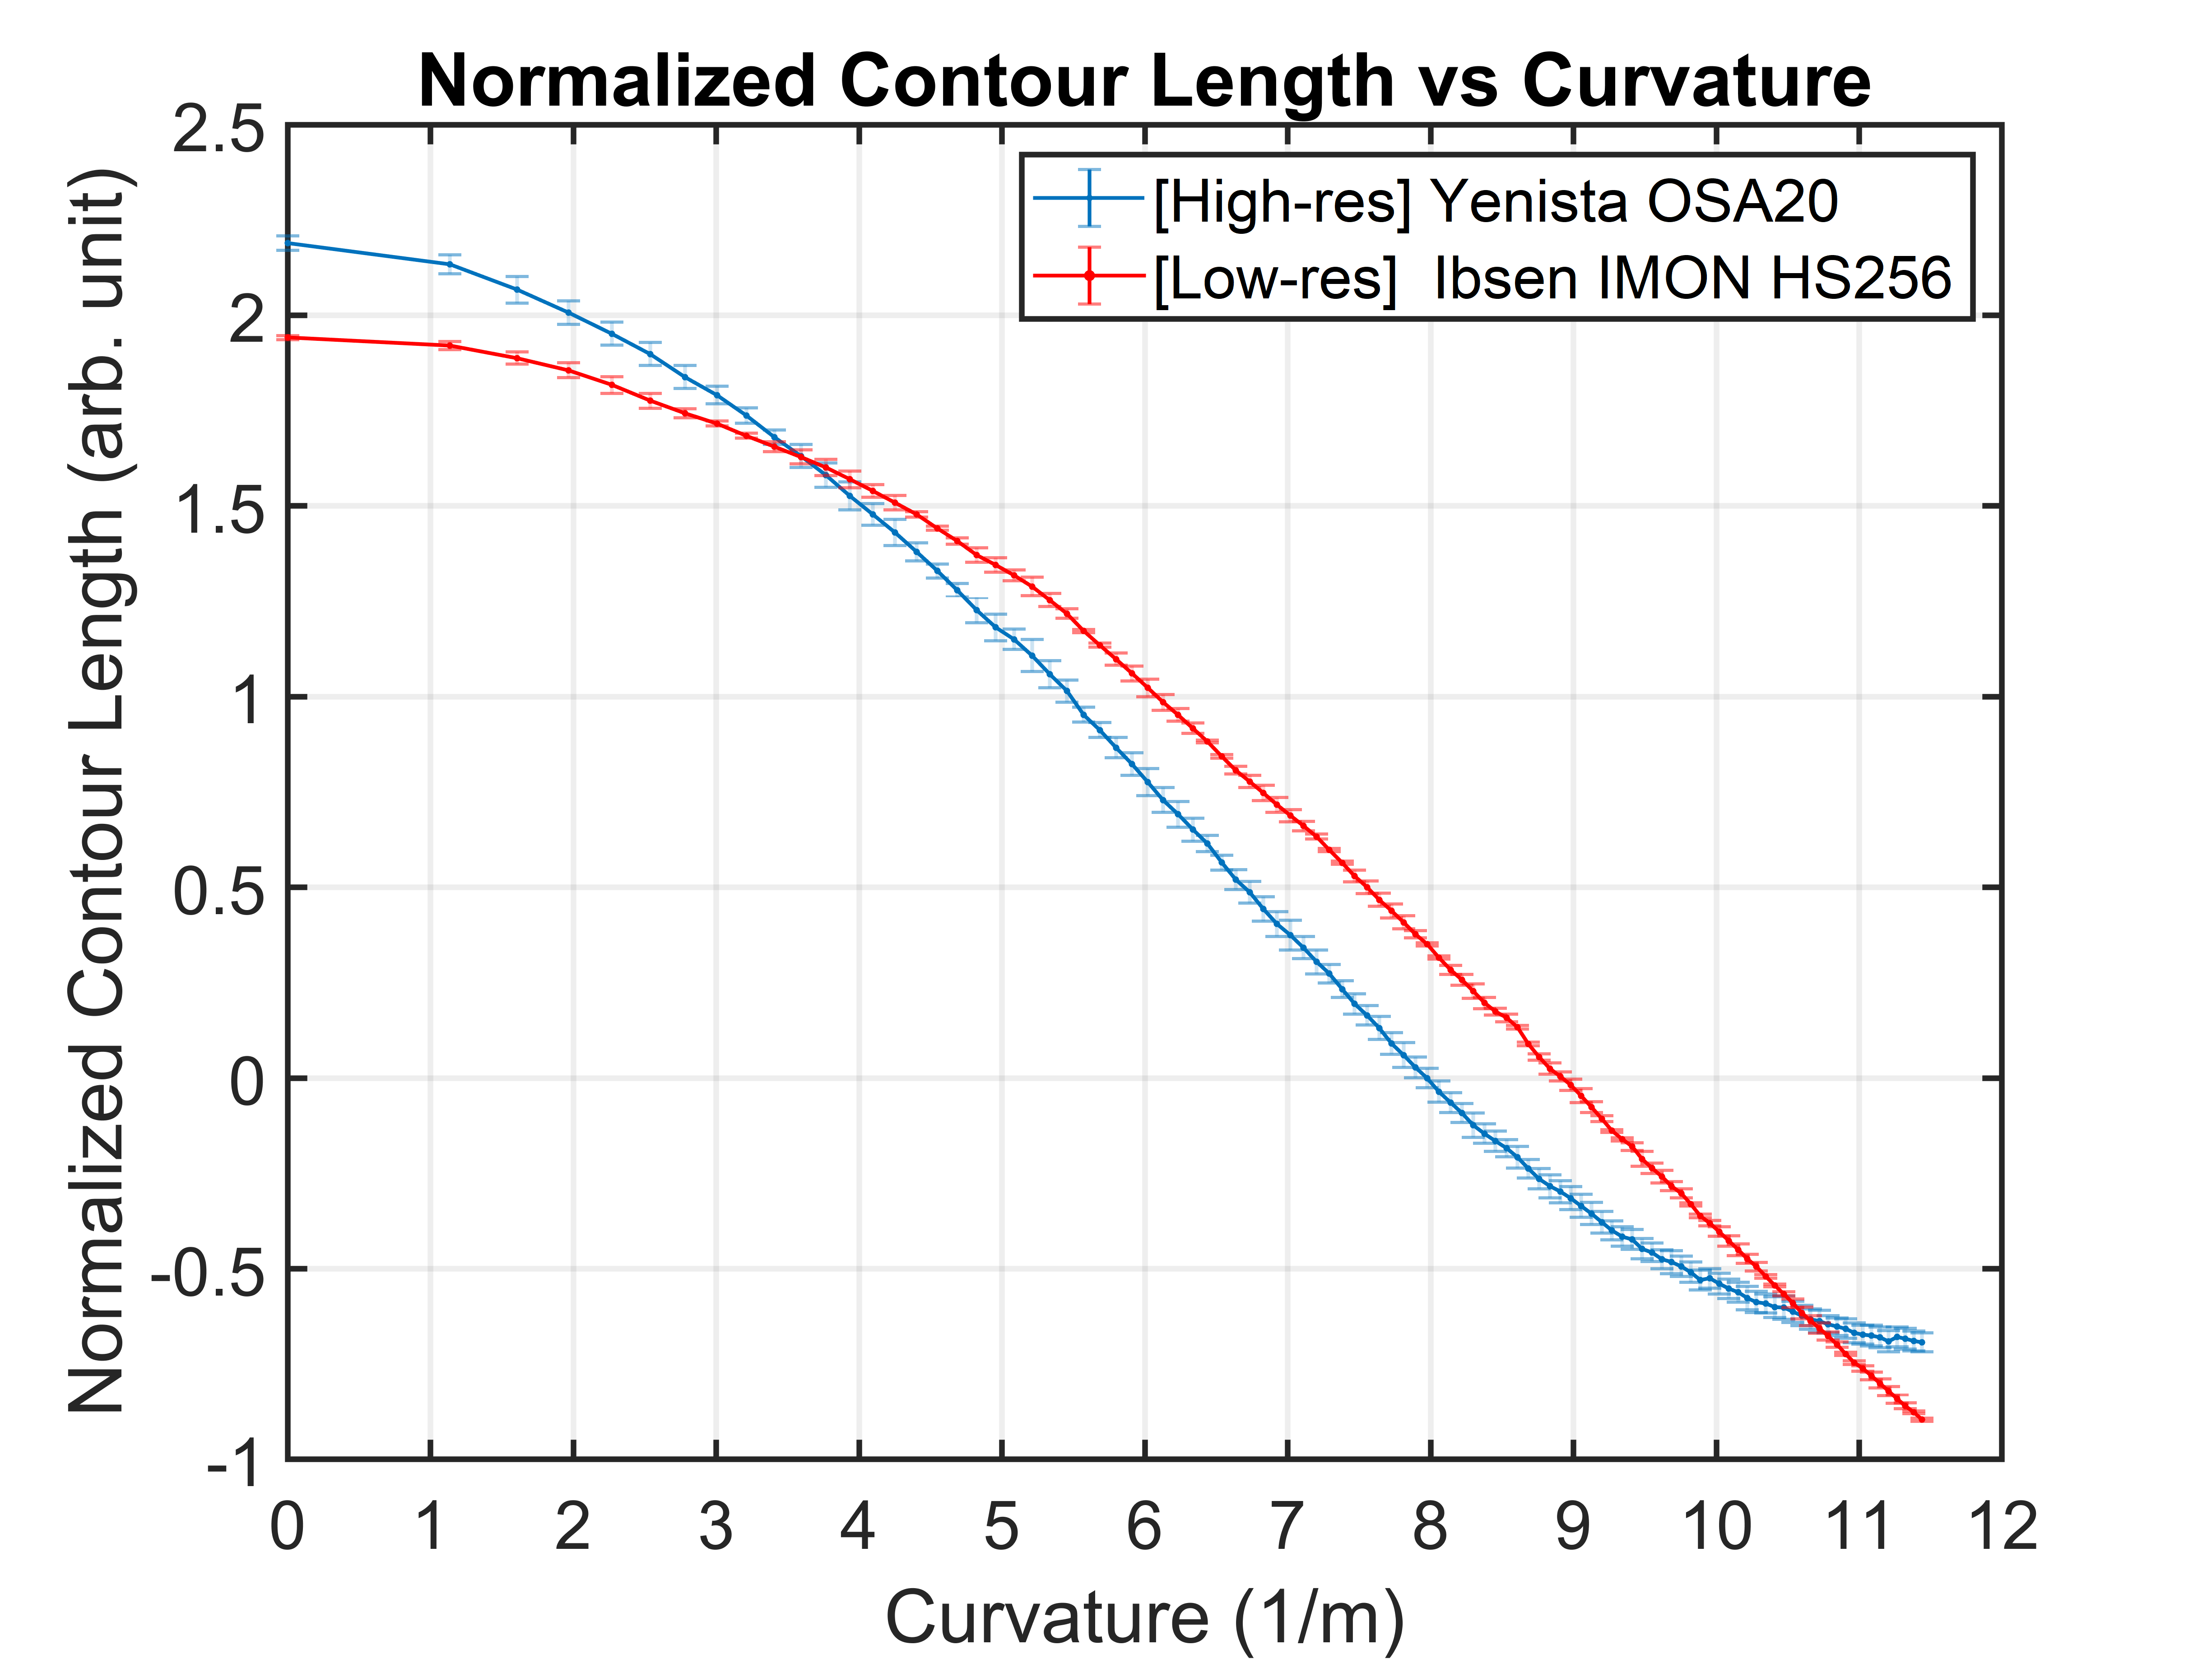
\includegraphics[width=1\linewidth]{Images/contour_len_curvature_HD_v3.png} 
\caption{Comparing equipment by applying CLA indicates high performance despite the low resolution.}
\end{figure}
\vspace{-0.3in}

%  ======= Vibration Sensing ============================================================

\begin{block}{Section 3} 

Lorem ipsum dolor sit amet, consectetur adipiscing elit. Donec lobortis orci felis, ut feugiat odio congue et. Praesent ut egestas quam. Mauris efficitur semper ornare proin.

\end{block}
\vspace{-0.3in}

\begin{figure}
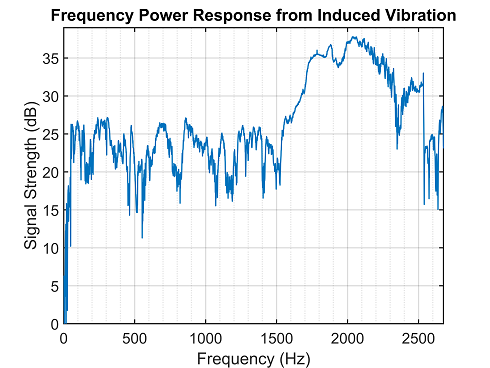
\includegraphics[width=1\linewidth]{Images/frequency_response_LQ.png}
\caption{A fiber in a fixed-fixed cavity (resonant frequency of \SI{2}{\kilo\hertz}) can detect external induced vibrations accurately.}
\end{figure}

%----------------------------------------------------------------------------------------

\end{column} % End of column 2.2

\begin{column}{\sepwid}\end{column} % Empty spacer column

\begin{column}{\onecolwid} % The first column within column 2 (column 2.1)

%----------------------------------------------------------------------------------------
% COLUMN 3
%----------------------------------------------------------------------------------------

%  ======= Surrounding Refractive Index Sensing =========================================

\begin{block}{Section 4}

Lorem ipsum dolor sit amet, consectetur adipiscing elit. Donec eleifend sollicitudin mauris. Nunc mollis gravida turpis, vel fermentum sem suscipit eu. Proin a elementum lorem. Suspendisse vulputate erat eu sapien consectetur, vitae aliquam metus sagittis. In hac habitasse platea dictumst. Vivamus cursus egestas sapien, sed imperdiet sapien mi.

\end{block}
\vspace{-0.3in}

\begin{figure}
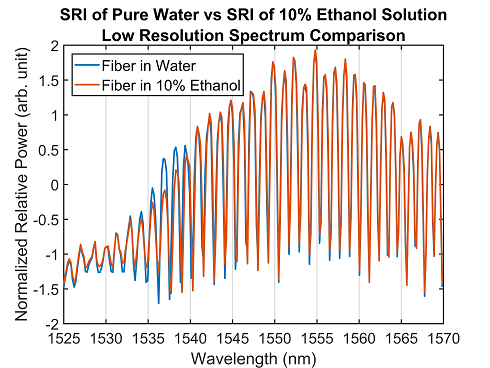
\includegraphics[width=1\linewidth]{Images/sri_spectrum_v2_LQ.png}
\caption{Ethanol has a slightly higher refractive index than water. This small increase leads to a large change in the TFBG spectra.}
\end{figure}
\vspace{-0.3in}

% \justifying{\fontfamily{lmr}\selectfont
% Praesent dictum tempor pulvinar. Suspendisse potenti. Sed tincidunt varius ipsum, et porta nulla suscipit et. Etiam congue bibendum felis, ac dictum augue cursus a. }\vspace*{1em}
% \vspace{-0.3in}

\begin{figure}
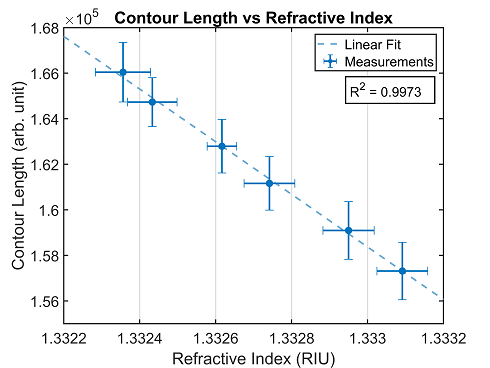
\includegraphics[width=1\linewidth]{Images/contour_len_ref_index_v2_HD_v2_LQ.png}
\caption{Using CLA on low-res data, an accuracy of $\pm\SI{83.5}{CLU}$ per \SI{d-4}{RIU} with 95\% confidence within $\pm\SI{0.024d5}{CLU}$ (Contour Length Units) was achieved.}
\end{figure}
\vspace{-0.3in}

%  ======= Conclusion ===================================================================

\begin{alertblock}{Conclusion}

Lorem ipsum dolor sit amet, consectetur adipiscing elit. Donec eleifend sollicitudin mauris. Nunc mollis gravida turpis, vel fermentum sem suscipit eu. Proin a elementum lorem. Suspendisse vulputate erat eu sapien consectetur, vitae aliquam metus sagittis. In hac habitasse platea dictumst. Vivamus cursus egestas sapien, sed imperdiet sapien mi.

\end{alertblock}
\vspace{-0.3in}

%  ======= References ===================================================================

\begin{block}{References}

\nocite{*} % Insert publications even if they are not cited in the poster
\small{\bibliographystyle{unsrt}
\bibliography{sample}\vspace{0.75in}}

\end{block}

%----------------------------------------------------------------------------------------

\end{column} % End of the third column

\end{columns} % End of all the columns in the poster

\end{frame} % End of the enclosing frame

\end{document}
